\begin{figure}[t]
\centering
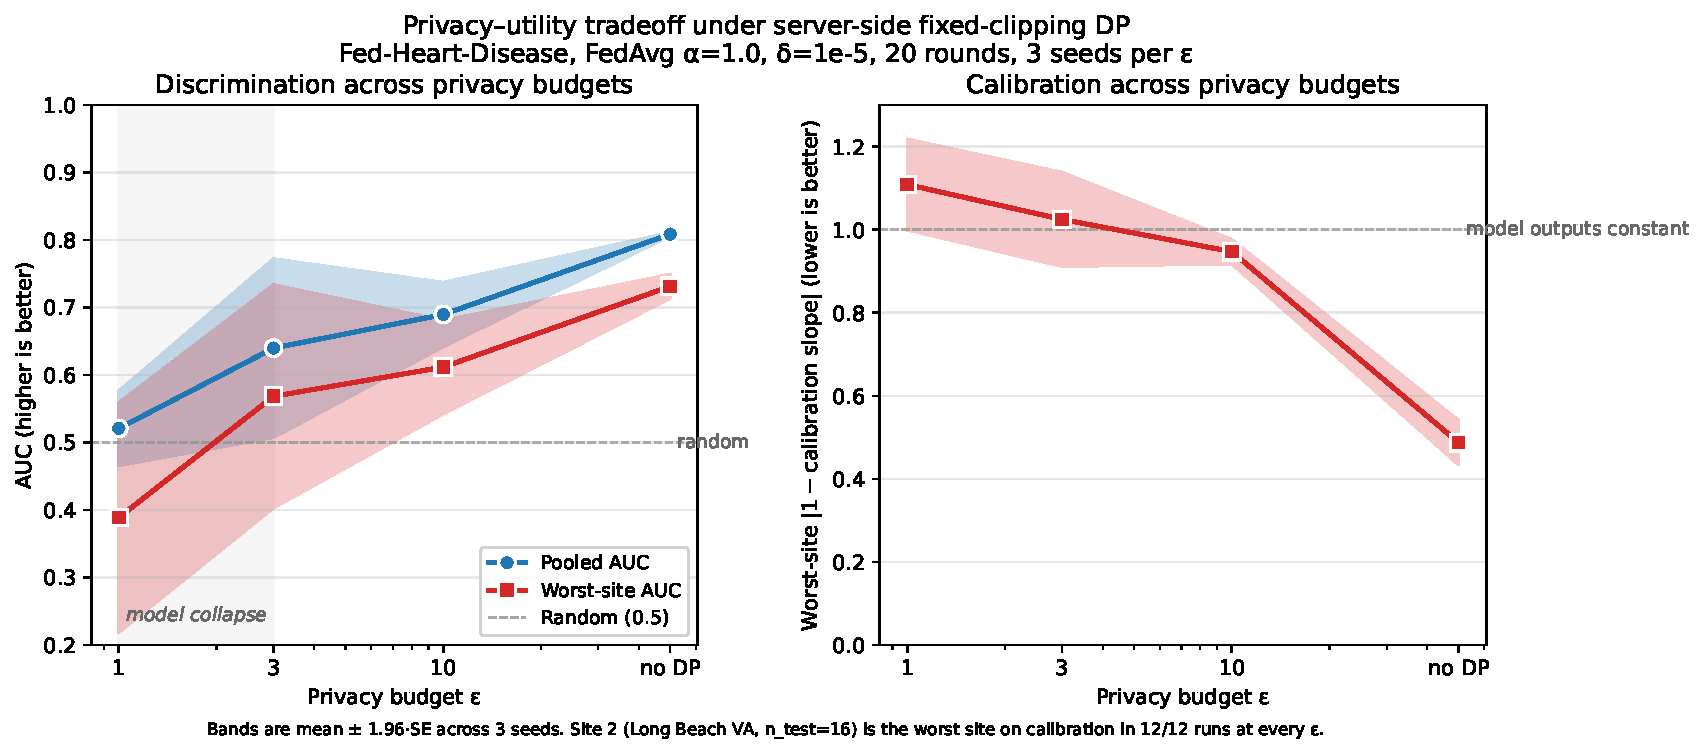
\includegraphics[width=\linewidth]{figures/exp5_dp_v2.pdf}
\caption{Privacy--utility tradeoff for the federated cardiovascular risk model under server-side fixed-clipping DP (Fed-Heart-Disease, FedAvg $\alpha{=}1$, $\delta{=}10^{-5}$, 20 rounds, 3 seeds per $\varepsilon$). \textbf{Left}: pooled AUC degrades by $36\%$ from no-DP to $\varepsilon{=}1$ while worst-site AUC degrades by $47\%$, and at $\varepsilon{=}1$ the worst-site AUC falls below random. \textbf{Right}: worst-site calibration slope deviation more than doubles, crossing the slope-deviation $=1.0$ threshold (model outputs constant) between $\varepsilon{=}10$ and $\varepsilon{=}3$. Bands are mean $\pm 1.96 \times$ SE across seeds. Site~2 (Long Beach VA, $n_{\text{test}}{=}16$) is the worst site on calibration in 12/12 runs.}
\label{fig:dp}
\end{figure}
